\documentclass[ProofPDF]{./Styles/Jnls-Template-V3}

\usepackage{amsmath}
\usepackage{array} % Required for m{} column
\usepackage{lineno}
% \usepackage{amssymb}

\newcommand{\CS}{\mathrm{CS}}
\newcommand{\INCB}{\mathrm{INCB}}
\newcommand{\IITT}{\operatorname{IITT}}
\newcommand{\ICS}{\operatorname{ICS}}

\newcommand{\intl}{\int\limits}
\newcommand{\suml}{\sum\limits}
\newcommand{\dd}[1]{\,\mathrm{d}#1}

\renewcommand{\vec}[1]{\mathbf{#1}}
\newcommand{\tens}[1]{\mathrm{#1}}
\newcommand{\itPhi}{\mathit{\Phi}}

% SI units
\usepackage{siunitx}
\DeclareSIUnit\year{yr}
\DeclareSIUnit\carbon{C}

% unit commands
\newcommand{\PgC}{\,\si{\peta\gram\carbon}}
\newcommand{\PgCyr}{\si{\peta\gram\carbon}\,\si{\year}}
\newcommand{\PgCperyr}{\si{\peta\gram\carbon}\,\si{\year}^{-1}}

% eqref with square brackets - shouldn't this work automatically by the chosen style?
\renewcommand{\eqref}[1]{Eq.~[\ref{#1}]}

% eqref without "Eq."
\newcommand{\noEqref}[1]{[\ref{#1}]}

% vector norm
\newcommand{\vnorm}[1]{\left\|#1\right\|}

\begin{document}

\jname{Tellus}
\jvol{00}
\jissue{00}
\jmonth{season}
\jyear{xxx}
\jid{doi}
\artid{xx.xxxx/xxxx.xx}
\filename{TISMIR\_LaTex\_Sample}
\def\MSFirstPage{\pageref{startPage_Label}}
\def\MSLastPage{\pageref{endPage_Label}}
\graphicspath{{./Images/}}
\label{startPage_Label}
%\title{Temporal integration of net ecosystem fluxes to assess multi-decadal carbon sequestration}
\title{Temporal integration of terrestrial net carbon fluxes reveals multi-decadal carbon debts due to previous carbon legacies}

\articletype{RESEARCH ARTICLE}

%\author[1]{Estefanía Muñoz}
%\rhauthor[1]{E. Muñoz}
%\howtociteauthor[1]{E. Muñoz}
%\author[2]{Holger Metzler}
%\author[3]{Marcos Fernández-Martínez}
%\author[4]{Jacob A. Nelson}
%\author[5]{Michael O'Sullivan}
%\author[6]{Stephen Sitch}
%\author[7]{Tobias Nützel}
%\author[8]{Jens Heinke}
%\author[9]{George Hurtt}
%\author[10]{Lei Ma}
%\author[11]{Qing Sun}
%\author[12]{Patrick C. McGuire}
%\author[13]{Etsushi Kato}
%\author[14]{Xiaojuan Yang}
%\author[15]{Wenping Yuan}
%\author[16]{Carlos A. Sierra}
%
%
%\aff[1]{CREAF, Cerdanyola del Vallès, Barcelona, Catalonia, Spain and Max Planck Institute for Biogeochemistry, Jena, Germany \href{mailto:e.munoz@creaf.uab.cat}{e.munoz@creaf.uab.cat}}
%\aff[2]{Department of Geography, Ludwig-Maximilians-Universität in Munich, Munich, Germany}
%\aff[3]{CREAF, Cerdanyola del Vallès, Barcelona, Catalonia, Spain}
%\aff[4]{Max Planck Institute for Biogeochemistry, Jena, Germany}
%\aff[5]{Faculty of Environment, Science and Economy, University of Exeter, Exeter, UK}
%\aff[6]{Faculty of Environment, Science and Economy, University of Exeter, Exeter, UK}
%\aff[7]{Department of Geography, Ludwig-Maximilians-Universität in Munich, Munich, Germany}
%\aff[8]{Potsdam Institute for Climate Impact Research (PIK), Leibniz Association, P.O. Box 60 12 03, 14412 Potsdam, Germany}
%\aff[9]{Department of Geographical Sciences, University of Maryland, College Park, MD 20770, USA}
%\aff[10]{Department of Geographical Sciences, University of Maryland, College Park, MD 20770, USA}
%\aff[11]{Climate and Environmental Physics, Physics Institute, University of Bern, Bern, Switzerland and Wyss Academy for Nature, University of Bern, Bern, Switzerland and Oeschger Centre for Climate Change Research, University of Bern, Bern, Switzerland}
%\aff[12]{Department of Meteorology \& National Centre for Atmospheric Science (NCAS), University of Reading, Reading, United Kingdom}
%\aff[13]{Institute of Applied Energy, Minato, Tokyo 105-0003, Japan}
%\aff[14]{Environmental Sciences Division, Oak Ridge National Lab, Oak Ridge, TN 37830, USA}
%\aff[15]{Institute of Carbon Neutrality, Sino-French Institute for Earth System Science, College of Urban and Environmental Sciences, Peking University, Beijing 100091, China}
%\aff[16]{Max Planck Institute for Biogeochemistry, Jena, Germany}
%
%\afflnote{*Author affiliations can be found in the back matter of this article}

\begin{history}
\submitted{\submittedday{xxx}\submittedmonth{xxx}\submittedyear{xxx}}
\accepted{\acceptedday{xxx}\acceptedmonth{xxx}\acceptedyear{xxx}}
\published{\publishedday{xxx}\publishedmonth{xxx}\publishedyear{xxx}}
\end{history}

\begin{abstract}[ABSTRACT]

%Land carbon sequestration fixes CO$_2$ from the atmosphere, storing it temporarily in terrestrial ecosystems. 
Carbon sequestration in terrestrial ecosystems is determined by how much carbon is assimilated by vegetation and how long that carbon remains stored before being released back into the atmosphere. The Carbon Sequestration (CS) metric integrates cumulative lag effects between assimilation and release, implicitly defined by transit times, providing a robust measure of both carbon amount and retention time. 
Here, we calculated CS by mathematically integrating carbon inputs and outputs from observation-based products (CarboScope, X-BASE, and CAMS) to quantify historical carbon legacies through assimilation rates and lagged releases tradeoffs associated with transit times. To explore longer timescales, we also computed CS using historical simulations from Earth System Models (CMIP6) and Dynamic Global Vegetation Models (TRENDY v13). Globally, assimilation rates and lagged releases are inversely related: tropical regions exhibit high assimilation rates but fast transit times, while high-latitude regions show lower assimilation rates but longer transit times. We found that high assimilation rates outweigh long transit times, rendering tropical regions the primary contributors to terrestrial carbon retention in the absence of disturbances. However, human activities such as land-use change have created a significant historical carbon debt relative to pre-industrial stocks, with cumulative releases exceeding newly stored carbon. Overall, this study highlights the importance of lag-time effects in understanding the terrestrial biosphere's capacity to store fossil-fuel-derived carbon and sustain the net land sink. It underscores how the choice of time horizon fundamentally shapes CS evaluations, highlighting the importance of accounting for carbon legacies.

\end{abstract}

\begin{keyword}[KEYWORDS:]

Climate change mitigation, Terrestrial ecosystems, Transit time, CarboScope, CAMS, X-BASE, CMIP6, TRENDY, 
\end{keyword}

\maketitle
\linenumbers

\section{Introduction}
The capacity of the biosphere to take up about a third of anthropogenic carbon emissions derived from the combustion of fossil fuels \citep{Ruehr2023,Friedlingstein2025} depends to a large degree on the long-term balance between its carbon inputs (assimilation) and outputs (release), which fluctuate over time and space due to natural processes and human activities \citep{Malhi1999}. Carbon inputs to terrestrial ecosystems are controlled by photosynthesis, while carbon outputs arise primarily from multiple respiration sources from vegetation and soils as well as disturbances \citep{Wisniewski1993, Trumbore2006}. 

Although there is good evidence that the terrestrial biosphere has acted as a significant sink of carbon during the previous decades \citep{Walker2021,Ruehr2023,Sitch2024}, there is large uncertainty regarding the stability and persistence of this sink \citep{Canadell2007,Fernandez-Martinez2023}. Radiocarbon provides a time‑stamped tracer of carbon that reveals how long carbon resides in terrestrial ecosystems before being returned to the atmosphere. For instance, measurements of atmospheric radiocarbon have shown that the terrestrial biosphere switched from a sink to a source of radiocarbon produced by thermonuclear-weapon testing about two decades after its spike in the atmosphere \citep{Naegler2009,Levin2022}. This shift suggests that carbon atoms transit rapidly ($\sim$ 2 decades) thorugh the terrestrial biosphere, and highlights the vulnerability of the land carbon sink and that net carbon uptake from the terrestrial biosphere is temporary. Similarly, recent radiocarbon measurements in ecosystem respiration have shown a one- to two-decade lag time between photosynthesis and respiration \citep{Tangarife2024JGR,Chanca2025,Sierra2026CCCR}, indicating that the large majority of carbon fixed by photosynthesis returns to the atmosphere in a matter of years to a few decades \citep{Sierra2023PTRS}. Therefore, the large land carbon sink could be overtaken by a lagged respiratory response that could reduce the sink strength or, under some scenarios, bring the land biosphere toward neutral or even positive net CO$_2$ fluxes.

A key metric to understand the temporary nature of the balance between carbon assimilation and release, as well as the lag times between carbon sinks and sources, is the transit time of carbon \citep{Thompson1999}. This metric characterizes the time elapsed from when carbon enters the system via photosynthesis until it is released back into the atmosphere. However, it is very difficult to determine it under the nonlinear and non-equilibrium conditions of the coupled carbon-climate system \citep{Rasmussen2016,Metzler2018PNAS}. Recent studies have shown that, for long periods (years to centuries), it is possible to obtain the cumulative lag effects between assimilation and release, implicitly defined by transit times, without explicitly computing this metric \citep{Metzler2024,Sierra2025}. This alternative approach relies on the time integration (double integral) of net carbon exchange, defined as the difference between instantaneous carbon inputs and outputs. This computation, which we define here as Carbon Sequestration (CS), can be applied to the large volumes of available information on net carbon fluxes between the land and the atmosphere derived from observational products and models. This formulation provides unique insights into the temporal dimension of carbon dynamics for assessing long-term (multi-decadal) carbon sequestration, which is not evident in the analysis of instantaneous fluxes or stock changes. A similar approach has been recently used by \citet{Matthews2023} and \citet{Metzler2024} to quantify the climate benefit of temporary carbon storage.

The central question motivating this work is whether the tradeoff between carbon assimilation and transit time favor long-term carbon sequestration in regions with high assimilation rates but fast carbon transit times (e.g., tropical ecosystems) or in regions with low assimilation rates but slow transit times (e.g., high-latitude ecosystems). This question arises because tropical forests exhibit large photosynthetic fluxes, yet carbon returns to the atmosphere relatively quickly (1-8 years) \citep{Sierra2021JE,Chanca2025}, whereas high-latitude ecosystems, despite lower photosynthetic rates, retain carbon for much longer ($>$100 years) \citep{Carvalhais2014,Lu2018}. While previous studies have characterized these baseline component fluxes independently, how their dynamic interaction controls the net, cumulative balance of historical carbon storage over decadal timescales remains a critical knowledge gap.

To address this question, we expand the analyses of \cite{Metzler2024} to global data-driven estimates of net carbon exchange between terrestrial ecosystems in the atmosphere, using bottom-up scaling products (X-BASE) and top-down atmospheric inversions (CarboScope, CAMS). We explored temporal tradeoffs between assimilation and release at the global scale over two decades, between 2001 and 2021. Then, to gain insights into longer timescales, we apply this methodology to process-based simulation output from Earth System Models (CMIP6) and Dynamic Global Vegetation Models (TRENDY v13), spanning the historical period since the beginning of the Industrial Revolution. 

By applying the CS framework across these different products, we aim to isolate the impacts of disturbance fluxes by directly comparing NEP- and NBP-based formulations of the CS metric. This comparison evaluates how disturbances, such as fire and land-use change, alter the tradeoffs between carbon uptake rates and transit times in terrestrial ecosystems. Furthermore, extending the analysis of CS back to 1850 using the process-based products allow us to track global carbon legacies, quantifying the historical carbon debt accumulated across distinct latitudinal zones.

\section{Datasets and methodology}\label{sec:methods}


\subsection{Datasets} 
% We calculated Carbon Sequestration (CS) using numerical outputs from three observation-based products and two model intercomparison products, using the variables Net Ecosystem Production (NEP) (or Net Ecosystem Exchange, NEE) and Net Biome Production (NBP).

%\subsubsection*{Observation-based products}
We calculated Carbon Sequestration (CS) using the monthly numerical outputs from two global atmospheric inversion models that assimilate CO$_2$ mole fraction data and provide gridded net land-atmosphere carbon exchange fluxes: CarboScope and CAMS. \hyperlink{https://www.bgc-jena.mpg.de/CarboScope/}{CarboScope} \citep[version nbetEXToc\_v2024E; ][]{Rodenbeck2005} provides daily flux estimates from 1957 to 2023 based on measurements at 173 sites, while \hyperlink{https://ads.atmosphere.copernicus.eu/datasets/cams-global-greenhouse-gas-inversion?tab=overview}{CAMS} \citep[v24;][]{Chevallier2013} provides monthly fluxes from 1979 to 2020 derived from over 100 surface measurement sites. Both products estimate land-atmosphere net carbon exchange by combining atmospheric CO$_2$ mole-fraction observations, atmospheric transport models, and constraints on anthropogenic carbon emissions and biospheric carbon exchange \citep{Kondo2022}. 

We treat these datasets as observation-based estimates of net biome production (NBP), recognizing that they constrain the net land–atmosphere CO$_2$ flux, which is dominated by biospheric exchange after accounting for fossil fuel and ocean fluxes. The number of sites contributing to these products has varied over time, with reported values reflecting the most recent simulations. While both products excel at capturing large-scale annual carbon growth rates and dynamic interannual climate anomalies, their top-down frameworks yield a coarse spatial resolution that cannot resolve localized, canopy-level dynamics. Furthermore, because their optimization routines rely on globally uneven observational networks, they exhibit higher spatial uncertainty and transport-model artifacts across data-scarce zones, particularly in the Global South\footnote{\color{blue} I prefer a geographical description rather than a political designation. There are regions in Siberia and Eurasia with low coverage that are not well capture in the designation of Global South} and tropical landmasses. 

In addition, we incorporated Net Ecosystem Exchange (NEE) estimates for 2001--2021 from the \hyperlink{https://meta.icos-cp.eu/collections/zfwf1Ak2I7OlziGDTX8Xl6_T}{X-BASE} product generated with FLUXCOM-X \citep{Nelson2024}. This machine-learning-based product integrates in-situ eddy covariance measurements, remote sensing data, plant functional types, and meteorological variables to deliver highly resolved, cloud-gap-free global NEE maps. Despite representing a major breakthrough for carbon cycle science, the dataset exhibits structural limitations. Specifically, its reliance on meteorological inputs causes it to underestimate interannual variability. Furthermore, sparse eddy covariance tower coverage in the Global South introduces regional artifacts across tropical and semi-arid zones, resulting in  false carbon sources in India and the Sahel and oversimplified moisture-stress responses in pristine tropical rainforests.


% FLUXCOM-X: NEE (0.5°, monthly)  01/2001-12/2021
% CarboScope: NBP (2.5° x 2°, daily) 01/1957-12/2023
% CAMS: NBP (1.4° x 0.7°, monthly) 01/1979,12/2020


%\subsubsection*{Model intercomparison products} 
To explore CS dynamics over more than a century of simulated history, we computed CS for 1850--2014 using monthly outputs of gross primary productivity (GPP), heterotrophic respiration (r$_h$), autotrophic respiration (r$_a$), and net biome production (NBP) from Earth System Models (ESMs) and Dynamic Global Vegetation Models (DGVMs). The ESMs were drawn from the sixth phase of the Coupled Model Intercomparison Project \citep[CMIP6; ][]{Eyring2016}. Eight models provided monthly NBP output, and eight supplied the remaining variables of interest (BCC-CSM2-MR lacks NBP outputs, and CESM2 does not provide monthly GPP, $r_a$, and $r_h$) for the {\it esm-hist} simulation (Table~S1). We used one ensemble member per model. These simulations span 1850-2014 and are forced by prescribed anthropogenic CO$_2$ emissions rather than CO$_2$ concentrations. Data were sourced from the German Climate Computing Centre \hyperlink{https://cmip-data-pool.dkrz.de/CMIP6-Data-Pool.html}{DKRZ}. We also incorporated results from 20 DGVMs compiled by the TRENDY v13 project \citep{Sitch2024}. Of these, 18 provided NBP outputs, and all 20 supplied GPP, r$_a$, and r$_h$ (Table~S2). We used experiment S3, which accounts for observed variations in atmospheric CO$_2$, land use change, and climate, and spans from 1700 to 2023. Despite well‑known discrepancies among such models, their simulations provide valuable insights into large‑scale carbon sequestration dynamics \citep{Gier2024,Sitch2024}.


%Data were requested through the \hyperlink{https://globalcarbonbudgetdata.org/closed-access-requests.html}{Global Carbon Budget}. 

CMIP6 and TRENDY models were included in the analysis to leverage their complementary strengths. TRENDY DGVMs focus on simulating terrestrial vegetation dynamics and ecosystem processes reconstructed from historical climate and land use, while CMIP6 ESMs provide a representation of the entire Earth system, including carbon-climate feedbacks, and often incorporate previous or current (sometimes simplified) versions of DGVMs used in TRENDY \citep{Argles2022,Weng2022}. For both CMIP6 and TRENDY models, NEP values are calculated as $\mathrm{NEP}=\mathrm{GPP}-(r_a+r_h)$.

Here, we assumed that NEE and NEP are interchangeable since both represent the same underlying processes—GPP minus respiration—despite being calculated using different data sources. Note that X-BASE, CAMS, and CarboScope follow an atmospheric convention: negative values denote CO$_2$ uptake by ecosystems, whereas CMIP6 and TRENDY use the opposite sign convention (positive for net carbon assimilation).

% NBP: LPJml, DLEM, LPJ-GUESS only have annual data.
% rh: LPJ-GUESS does not have it. 
% CARDAMOM was removed to calculate the weights and the ensemble because it only has data from 2003.

\subsection{Homogenization and ensemble calculations}
To enable comparison, data from all products were regridded to a uniform $1^\circ\times1^\circ$ spatial resolution using the bilinear interpolation method implemented via \hyperlink{https://xesmf.readthedocs.io/}{xESMF \citep{zhuang2023}}. Datasets with higher temporal resolutions were standardized to monthly averages. For calculations using observation-based products, we homogenized the time series for the period 01-2001 to 12-2019, while for CMIP6 and TRENDY we employed the full historical simulation period of CMIP6, i.e., 1850--2014. To compare all products, we selected the 2001--2014 period, during which all datasets overlap.
Positive NEP and NBP values were defined as fluxes moving from the atmosphere to the land surface, which contrasts with the conventions used in inverse models.

We computed CMIP6 and TRENDY ensemble averages using a pixel-scale, performance-based weighting scheme instead of a simple equal-weight mean. This approach, described in \citet{Sierra2025GDM}, follows the multimodel inference framework of \citet{Burnham2002} (building on Akaike’s 1970s work) and calculates each model's weight by measuring its relative distance from observed data, approximating the Kullback-Leibler distance between models and the unknown reality at the pixel scale. Because direct global observations are unavailable, we used data-driven products derived from sparse measurements and extrapolated to the terrestrial surface. Specifically, we used X-BASE (2001-2021) to assign model weights for NEP and CarboScope (1957-2023) to assign weights for NBP averages, selecting CarboScope over CAMS due to its longer time series. 
%Both models and data-driven products should have the same spatial and temporal coordinates.
 
For each model $i$, observational product $j$, and spatial coordinate $s$, we computed the mean squared deviation ($\hat\sigma^2_{i-j, s}$) between model output and  observational product over their overlapping period. Model weights ($w_{i-j, s}$) were then defined as the normalized inverse of these deviations
\begin{equation}
    w_{i-j, s}=\frac{1/\hat\sigma^2_{i-j, s}}{\sum^k_{r=1}1/\hat\sigma^2_{r-j, s}},
\end{equation}
for the $k$ models in the ensamble. 

Thus, models closer to the observational product at a given pixel receive larger weights, with the weights normalized such that $\sum_s w_{i-j, s}=1$.

Although the observational products $j$ cover only part of the simulation period (X-BASE:2001--2014, CarboScope:1957--2014), we applied the resulting static (time-invariant) pixel weights across the full time span of the ESM and DGVM simulations. This assumes that a model performing well during the observation window will also perform relatively well in other periods. While this assumption is not perfect, it is more defensible than assuming all models are equally reliable at all times, as an equal-weight ensemble implicitly does. These fixed weights were then used to compute spatially explicit time-dependent ensemble means ($\overline{x}_{j, s, t}$) for CMIP6 and TRENDY models (Figs.~S4-S7) as
\begin{equation}
   \overline{x}_{j, s, t} =\sum_{i=1}^{k}w_{i-j, s} \cdot x_{i, s, t},
\end{equation}
where $t$ is the time index, and $x$ are the values of the variable of interest (NEP or NBP).

The resulting ensemble maps do not simply select the “best” model everywhere. Instead, at each grid cell they combine contributions from all models, with larger influence from those with smaller deviations from the observational product. As shown in \citet{Sierra2025GDM}, no single CMIP6 ESM performs best (or worst) globally for either NEP or NBP, and this performance-based weighting yields substantially lower uncertainty estimates than equal weighting. Two limitations remain: inter-model dependence is not explicitly accounted for, and there is no penalty for model complexity.%, as in formal information-theoretic model selection.
 
% using all data from periods that overlap with the available data periods of CarboScope (CMIP6:1957-2014, TRENDY:1957-2023) or FLUXCOM-X (CMIP6:2001-2014, TRENDY:2001-2021) (\textcolor{red}{see Supplementary Figs.~1-4}).


% Units:
% CMIP6: kg m${-2}$ s${-1}$.
% TRENDY: kg m${-2}$ s${-1}$.
% FLUXCOM-X: g m${-2}$ d${-1}$.
% CarboScope: PgC yr${-1}$
% CAMS: g m${-2}$ s${-1}$.


\subsection{Carbon sequestration} 
Carbon sequestration (CS) is defined here as the accumulated uptake or loss of carbon in terrestrial ecosystems over time, which can be obtained as the integral of carbon storage over time \citep{Sierra2021}. This definition is equivalent to the double integral of the net carbon flux between the atmosphere and the terrestrial biosphere over a defined period starting at a reference year $t_0$ over a fixed time horizon $T$ \citep{Sierra2021,Metzler2024,Sierra2025}, as
\begin{equation} \label{eq:CS}
    \mbox{CS}\left(t_0,T\right):=\int^{t_0+T}_{t_0} \int^{t}_{t_0} \left[s(t')-r(t')\right]\mathrm{d}t'\mathrm{d}t,
\end{equation}
where $s(t')$ is the gross flux rate of carbon removed from the atmosphere at a given time $t$, and $r(t)$ is the gross flux rate of carbon released from the terrestrial surface back to the atmosphere. The prime symbol ($'$) in the equation represents a dummy variable for integration. This definition of CS accounts for both the fate of new carbon inputs and the legacy carbon already present in the system at $t_0$ \citep{Metzler2024}. It combines the amount of mass that enters the ecosystem with the time carbon remains stored (see Fig.~1 in \citet{Munoz2024}). In \ref{sec:appCS}, we mathematically demonstrate that the CS definition in \eqref{eq:CS} implicitly accounts for the transit time of carbon in ecosystems, a very difficult metric to compute from observations or model output.

Geometrically, CS represents an area with mass and time as its primary components. It results from the temporal double integration of net carbon fluxes (mass/time $\times$ time $\times$ time) (see ~\ref{tab:family_of_measures}), so its results are reported in units of PgC~yr. Positive CS values should be interpreted as a situation in which the cumulative amount of carbon retained by the terrestrial biosphere exceeds the cumulative amount released over the evaluation period. Negative CS values indicate the opposite—more carbon has been released than retained during the period—signifying a carbon debt relative to previous storage levels and reflecting accumulated losses over time.

When calculating global Carbon Sequestration or aggregating it by latitudinal zones, the grid areas were factored into the computation, removing spatial units. Latitudinal zones are defined as tropical: 22.5$^\circ$S--22.5$^\circ$N, mid-latitudes: 22.5$^\circ$S--55.0$^\circ$S and 22.5$^\circ$N--55.0$^\circ$N, and high latitudes: $>$55.0$^\circ$N.

\subsection{Carbon disturbance fluxes}

Carbon Sequestration was calculated using both Net Ecosystem Production (NEP) and Net Biome Production (NBP). NEP represents the net carbon exchange between ecosystems and the atmosphere, whereas NBP further accounts for large-scale disturbances such as fires and logging, and lateral carbon transfers like riverine export. This distinction allows for analysis of the impacts of these processes on CS. 

CarboScope and CAMS provide net land-atmosphere CO$_2$ fluxes that implicitly include all processes affecting atmospheric CO$_2$: natural biospheric fluxes, anthropogenic land-use fluxes, and biomass burning emissions, to the extent that they are either prescribed in the prior fluxes or inferred from the atmospheric CO$_2$ signal. In addition, CAMS explicitly prescribes GFAS (Global Fire Assimilation System) fire emissions as the prior for biomass burning. The net land exchange delivered by these inversion products is therefore physically equivalent to NBP.

X-BASE provides upscaled NEE derived from eddy-covariance tower measurements. Although these measurements may implicitly reflect local disturbances occurring at the sites, X-BASE does not include explicit modules or input data to track wildfire combustion emissions or land-use conversion events. As mentioned before, NEE is functionally comparable to NEP.

CMIP6 ESMs and TRENDY DGVMs provide both NEP and NBP, with the representation of disturbance fluxes depending on the individual model and its land-surface scheme.


\section{Results}

\subsection{Two-decade Carbon Sequestration in the absence of disturbances}
Carbon Sequestration (CS), calculated as the double temporal integral of NEP (Eq.~\ref{eq:CS}) from X-BASE, reveals a predominantly positive global distribution, with notable exceptions in hyper-arid zones (Fig.~\ref{fig:CS_NEP}a). However, the pronounced negative values observed in India are recognized as structural artifacts reflecting known product limitations in that region. Areas dominated by forests exhibit the highest CS values, particularly across the Amazon basin, eastern and western North America, the Congo basin, Western Europe, and Southeast Asia. The latitudinal CS profile (Fig.~\ref{fig:CS_NEP}b) demonstrates positive CS across most latitudes, except for latitudes around 20--30$^{\circ}$S and 18--35$^{\circ}$N, indicating sustained zonal carbon sequestration over the 2001--2019 period. Peak CS occurs in tropical latitudes (approximately 22$^{\circ}$S to 18$^{\circ}$N) and at around 30--40$^{\circ}$S, whereas mid-latitudes show zero or negative values.

Although high latitudes sequester more carbon per unit area on average than mid-latitudes (Fig.~\ref{fig:CS_NEP}b), the larger territorial expanse of mid-latitudes results in a higher total CS (Fig.~\ref{fig:CS_NEP}c). When accumulating CS by latitudinal zones over time (Fig.~\ref{fig:CS_NEP}c), the divergence among zones increases, reflecting the capacity of the tropics to sequester carbon in the absence of disturbances. The higher CS values in tropical and boreal regions compared to mid-latitudes suggest that either high carbon assimilation or slow carbon releases contribute to long-term carbon retention, but the dominant role of high carbon assimilation is evident (Figs.~S1 and S2), as reflected by the high, sustained positive CS values observed in the tropics. 

\begin{figure*}
    \centering
    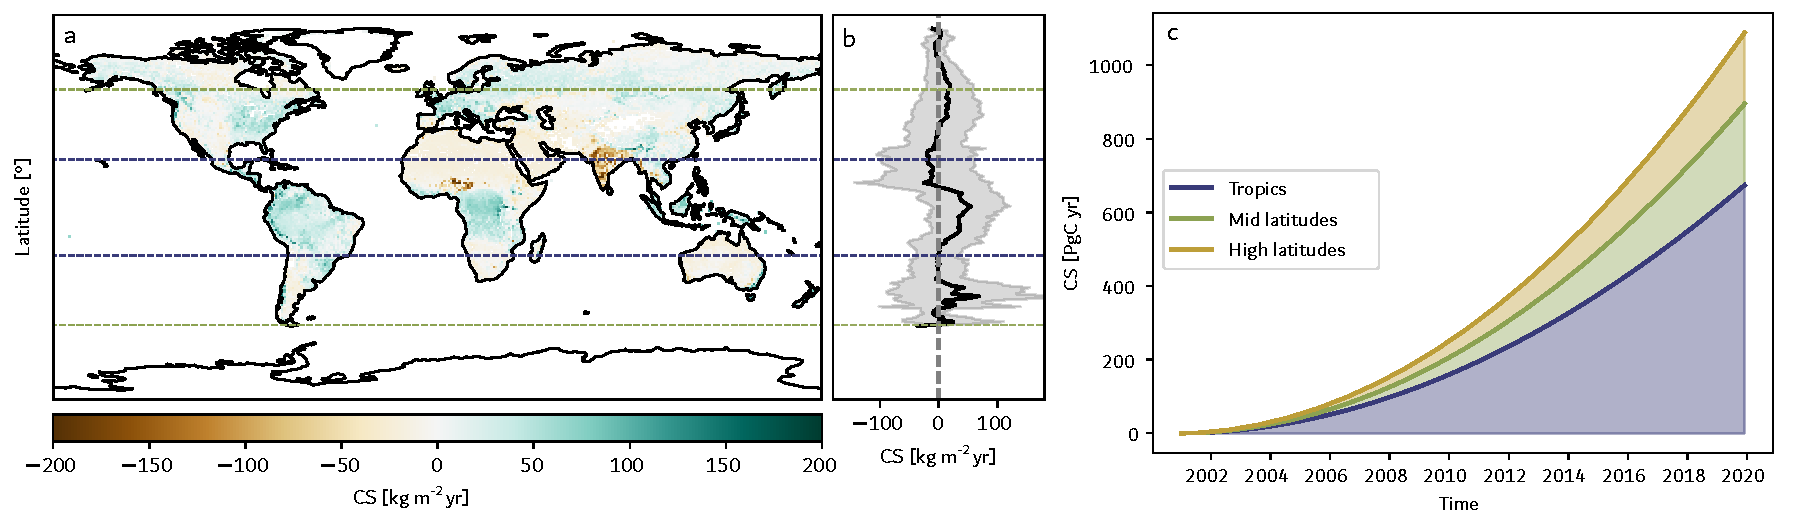
\includegraphics[width=1.0\textwidth]{Images/NEP_obsprod_compressed.pdf}
    \caption{a) Global map of Carbon Sequestration (CS), b) latitudinal CS profile (mean), and c) temporal trends of global cumulative CS alongside the contribution of latitudinal zones (indicated by colors), derived from NEP in the X-BASE product for 2001--2019. Horizontal dotted lines in a and b delimit the tropical, mid latitudes, and high latitudes zones. The vertical dashed line in b represents null values of CS, and the shadow areas indicate two standard deviations around the spatial mean.}
    \label{fig:CS_NEP}
\end{figure*}

\subsection{Disturbance impacts on Carbon Sequestration integrated over two decades}

The previous results, derived from the double integral of NEP, capture only the tradeoff between GPP and ecosystem respiration, excluding additional CO$_2$ emissions from disturbances like deforestation and fires. When CS is calculated from the double integral of Net Biome Production (NBP)—which incorporates these additional disturbance emissions—spatial and temporal dynamics change markedly, with values about an order of magnitude smaller than those obtained with NEP (Figs.~\ref{fig:CS_NEP} and \ref{fig:CS_NBP}). Both CarboScope and CAMS show a pronounced CS peak near 50$^{\circ}$N and very low values in tropical regions (Fig.~\ref{fig:CS_NBP}b,e), including negative or near-zero values across the Amazon and Congo basins (Fig.~\ref{fig:CS_NBP}a,d). While the NEP-based CS from X-BASE identifies the tropics as the zones with the highest CS values, reaching 674 PgC~yr over 2001--2019 (Fig.~\ref{fig:CS_NEP}c), the NBP-derived CS indicates these regions have the lowest values or even negative values—according to CAMS, -78 PgC~yr (Fig.~\ref{fig:CS_NBP}f)— reflecting a net carbon debt relative to 2001, where cumulative losses exceed carbon gains. Globally, the differences between NEP-based and NBP-based CS reach 780~PgC~yr for CarboScope and 624~PgC~yr for CAMS, with tropical regions contributing 82\% (646~PgC~yr) and 121\% (756~PgC~yr) of these differences, respectively. At mid and high latitudes, CarboScope indicates lower NBP-based CS than NEP-based CS estimates (reductions of 46\% and 19\%, respectively), whereas CAMS suggests increases of 41\% and 19\%, respectively. 

\begin{figure*}
    \centering
    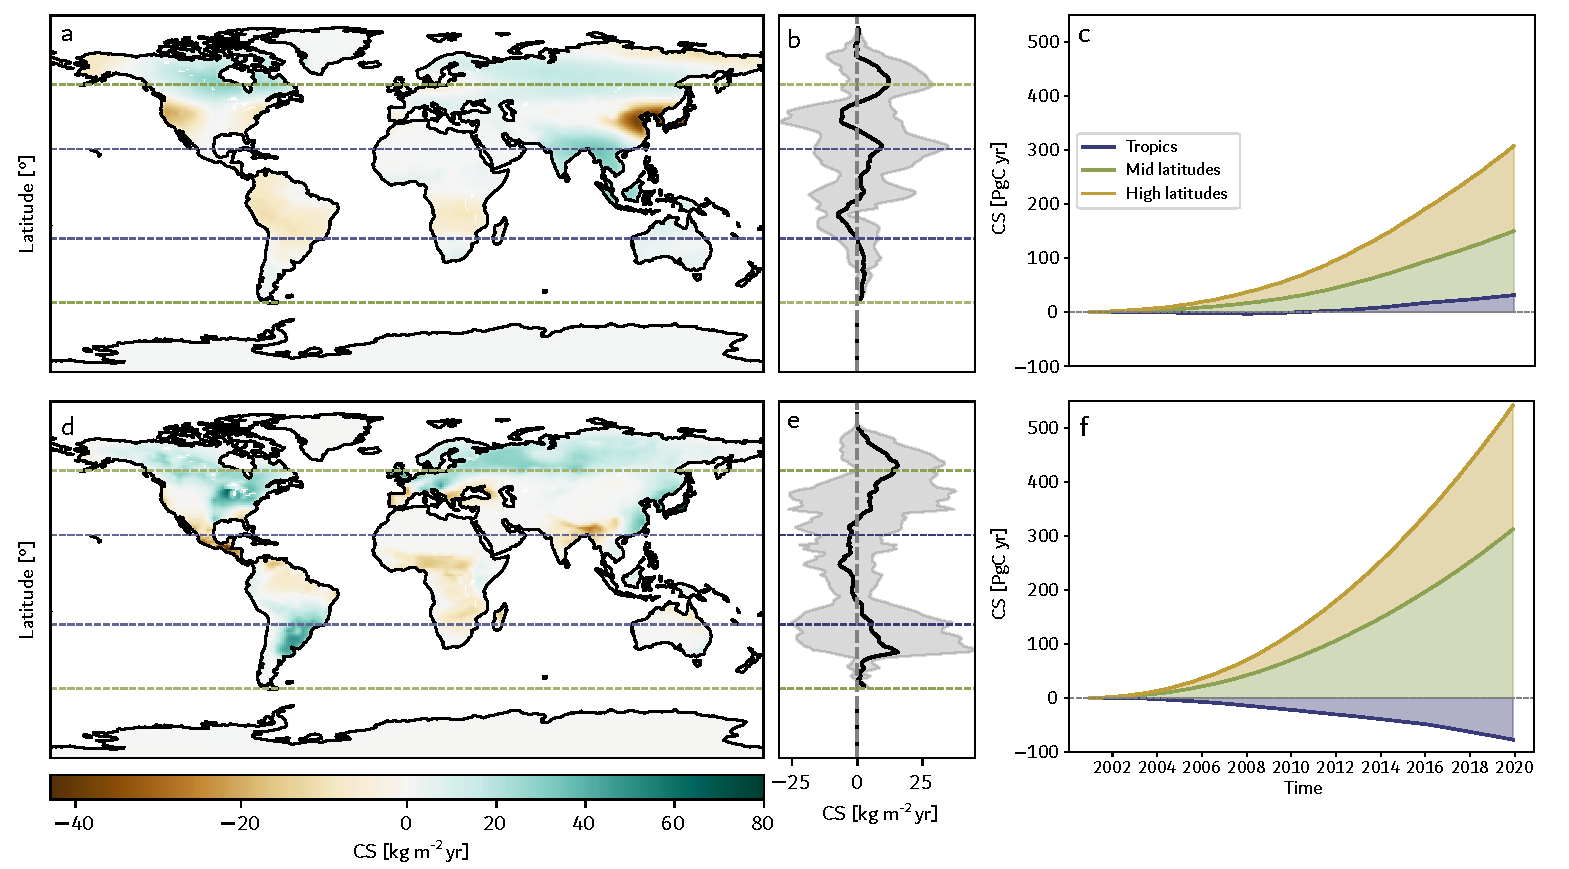
\includegraphics[width=1.0\textwidth]{Images/NBP_obsprod_compressed.pdf}
    \caption{a,d) Global map of Carbon Sequestration (CS), b,e) latitudinal CS profile (mean), and c,e) temporal trends of global cumulative CS alongside the contribution of latitudinal zones (indicated by colors), derived from NBP in the CarboScope (a--c) and CAMS (d--f) products for 2001--2019. Horizontal dotted lines in a,b,d and e delimit the tropical, mid latitudes, and high latitudes zones. The vertical dashed lines in b and e represent null values of CS, and the shadow areas indicate two standard deviations around the spatial mean.}
    \label{fig:CS_NBP}
\end{figure*}



\subsection{Carbon Sequestration and disturbance impacts integrated over 165 years} 

Carbon Sequestration derived from NEP using CMIP6 and TRENDY output consistently show an upward and increasing trend across latitudinal zones over time, albeit with varying magnitudes (Fig.~\ref{fig:CMIP6_TRENDY_NEP_time}). The CMIP6 ensemble yields a larger global CS for 1850--2014 compared to the TRENDY ensemble (7.7$\times$10$^{4}$ vs. 3.9$\times$10$^{4}$~PgC~yr). Yet, both ensembles agree that tropical regions retained the largest amount of carbon between 1850 and 2014, followed by mid-latitudes (Fig.~\ref{fig:CMIP6_TRENDY_NEP_time}a,c). All models indicate positive CS values in the tropics throughout the studied period, though two CMIP6 models (BCC-CSM2-MR and CanESM5) and one TRENDY model (ED) show negative CS in mid-latitudes, and three CMIP6 models (BCC-CSM2-MR, CanESM5 and UKESM1-0-LL) and two TRENDY models (ED and DLEM) in high-latitudes (Fig.~\ref{fig:CMIP6_TRENDY_NEP_time}c,d). 

\begin{figure}
    \centering
    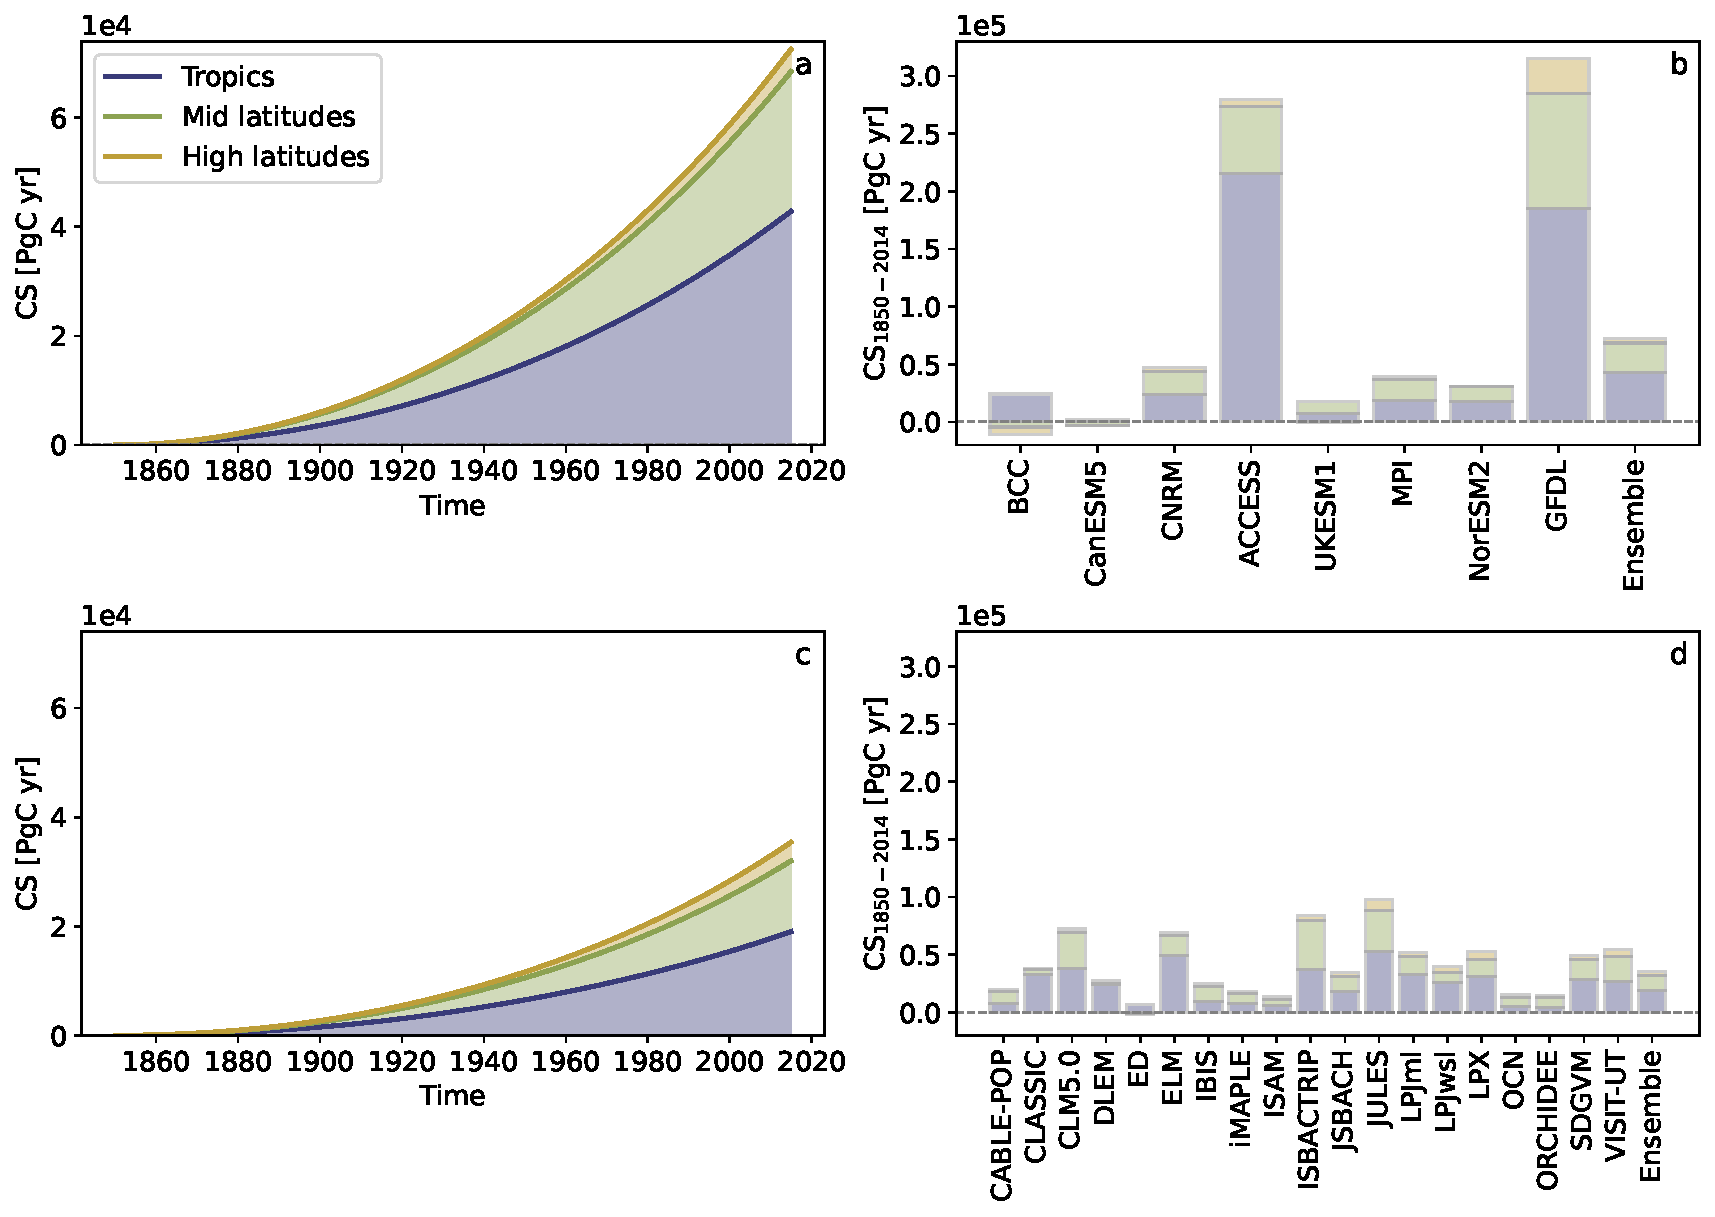
\includegraphics[width=1.0\linewidth]{Images/NEP_CMIP6_TRENDY_CS_time_final_res.pdf}
    \caption{Temporal trends in Carbon Sequestration (CS) (a,c) and CS at the end of the period from 1850 to 2014 (b,d) calculated using NEP from CMIP6 (a,b) and TRENDY (c,d), and the contributions of latitudinal zones (colors). Panels a and c show results from the CMIP6 and TRENDY models' average ensemble, respectively, and panels b and d show results for each model alongside the ensemble. The dotted lines represent null CS values, with negative (positive) values indicating carbon debts (surpluses). To optimize space, only the initial part of each model name is displayed on the horizontal axes in b.}
    \label{fig:CMIP6_TRENDY_NEP_time}
\end{figure}

When disturbances are included (NBP-based), spatial and temporal dynamics change markedly, with values mainly negative (Fig.~\ref{fig:CMIP6_TRENDY_NBP_time}). Positive values occur but are roughly two orders of magnitude smaller than NEP-based estimates (Fig.~\ref{fig:CMIP6_TRENDY_NEP_time}). Negative values reflect a net carbon debt relative to pre-industrial stocks over the 165-year period, where cumulative losses exceed carbon gains. Both ensembles simulate global net debts, with larger magnitudes in CMIP6 than in TRENDY (-2.8$\times$10$^{3}$~PgC~yr vs. -1.1$\times$10$^{3}$~PgC~yr). CMIP6 ensemble shows negative CS across all latitudinal zones, whereas TRENDY produces negative values only in mid-latitudes, maintaining low positive values elsewhere compared to NEP-based estimates (Fig.~\ref{fig:CMIP6_TRENDY_NBP_time}a,c). 

\begin{figure}
    \centering
    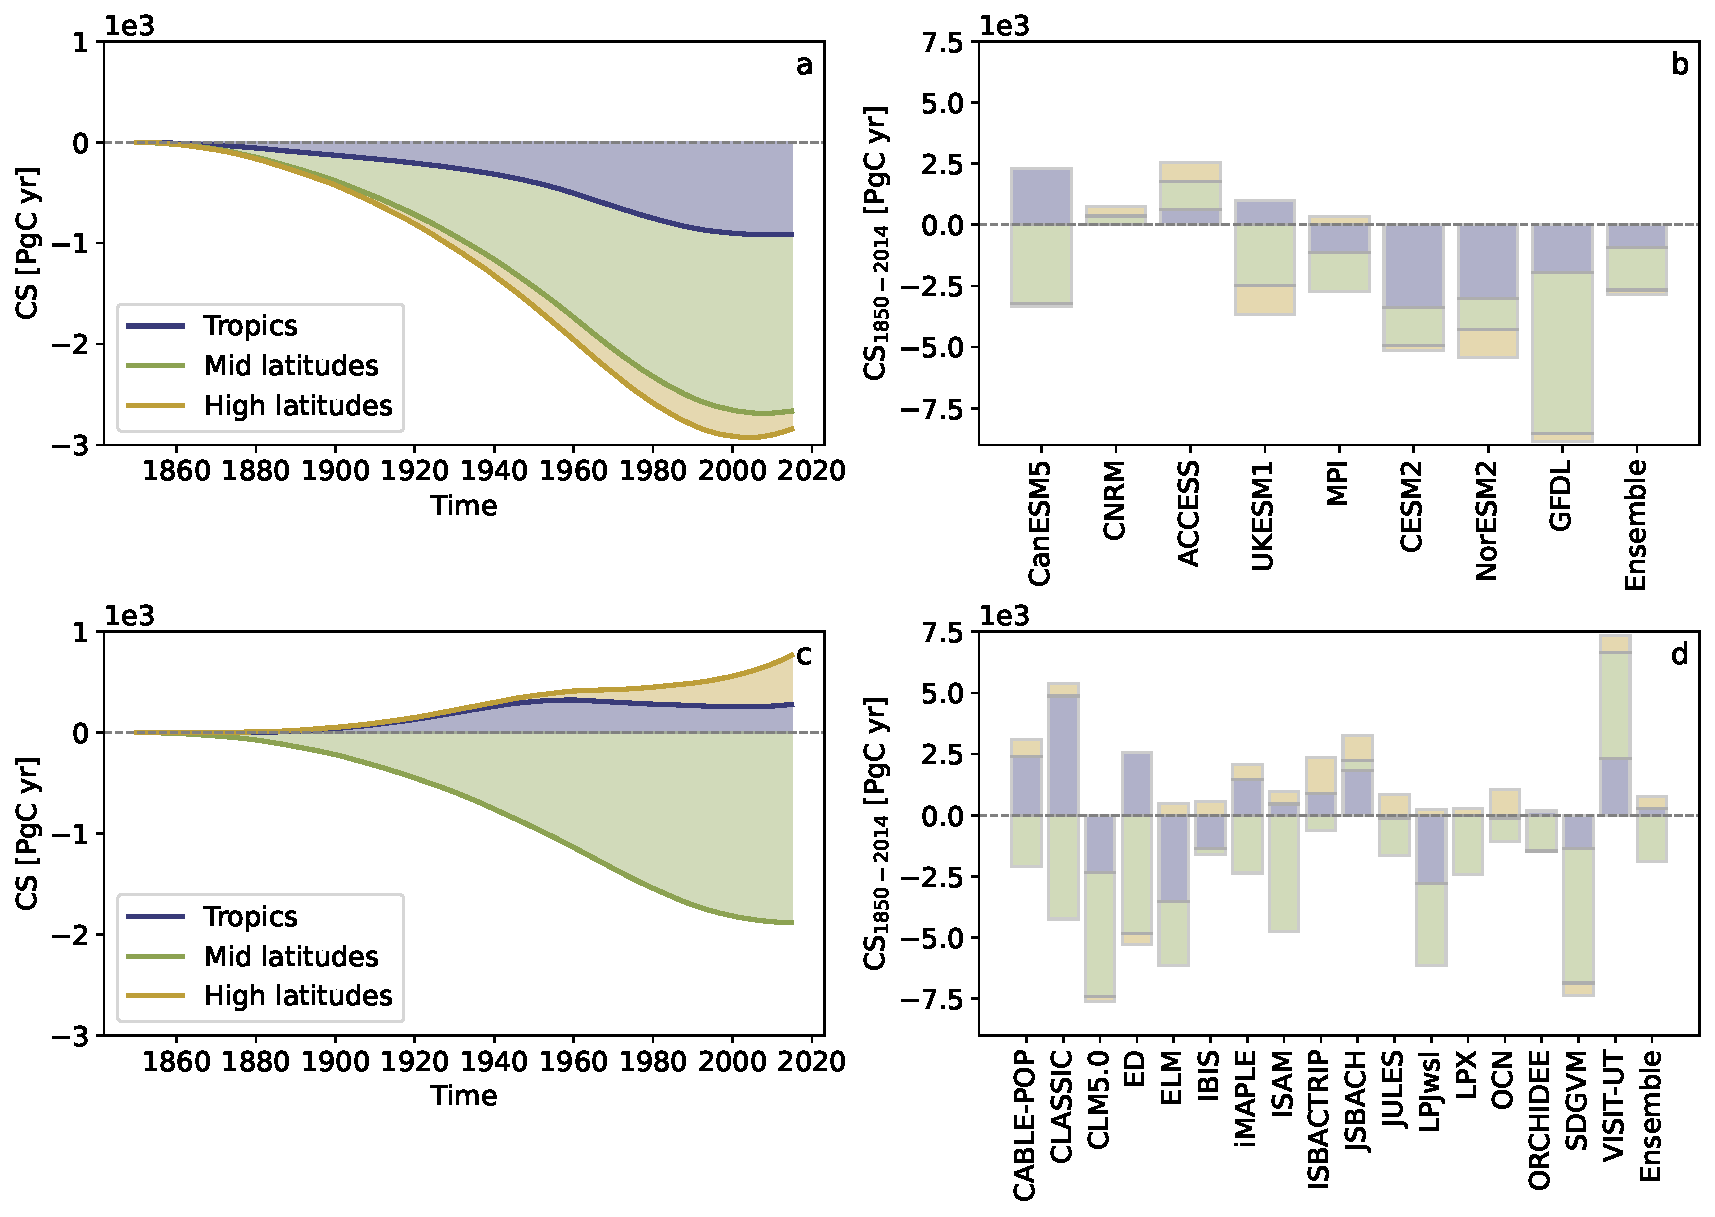
\includegraphics[width=1.0\linewidth]{Images/NBP_CMIP6_TRENDY_CS_time_final_res.pdf}
    \caption{Temporal trends in Carbon Sequestration (CS) (a,c) and CS at the end of the period from 1850 to 2014 (b,d) calculated using NBP from CMIP6 (a,b) and TRENDY (c,d), and the contributions of latitudinal zones (colors). Panels a and b show results from the CMIP6 and TRENDY models' average ensemble, and panels b and d show results for each model alongside the ensemble. The dotted lines represent null CS values, with negative (positive) values indicating carbon debts (surpluses). To optimize space, only the initial part of each model name is displayed on the horizontal axes in b.}
    \label{fig:CMIP6_TRENDY_NBP_time}
\end{figure}

Across latitudinal zones, the CMIP6 ensemble shows the least negative CS at high latitudes, followed by the tropics (Fig.~\ref{fig:CMIP6_TRENDY_NBP_time}a). Similarly, the TRENDY ensemble shows that high-latitude regions have the highest values, followed by the tropics (Fig.~\ref{fig:CMIP6_TRENDY_NBP_time}c). In both ensembles, mid-latitudes exhibit the most negative CS values over the studied period. Interestingly, unlike the monotonically increasing NEP-based CS trend, the NBP-based CS trajectory from the CMIP6 ensemble declines from 1850 to around 1970, followed by a modest recovery in recent decades (Fig.~\ref{fig:CMIP6_TRENDY_NBP_time}a). The TRENDY ensemble shows a similar pattern in mid-latitudes, a positive slope in high latitudes, and near-stable values in the tropics (Fig.~\ref{fig:CMIP6_TRENDY_NBP_time}c). Most CMIP6 models simulate negative global CS, except CNRM-ESM2-1 and ACCESS-ESM1-5, while in TRENDY, only CABLE-POP, CLASSIC, ISBACHTRIP, JSBACH, and VISIT-UT show positive global CS. Nearly all models yield negative CS in mid-latitudes except CNRM-ESM2-1 and ACCESS-ESM1-5 (CMIP6) and JSBACH and VISIT-UT (TRENDY). Results are more variable in the tropics and high latitudes, particularly within TRENDY models (Fig.~\ref{fig:CMIP6_TRENDY_NBP_time}b,d). 

The difference between NEP- and NBP-based CS is dominated by tropical regions. Globally, CS differs by 75359~PgC~yr in CMIP6 and 36523~PgC~yr in TRENDY, with tropical regions accounting for 58\% (43722~PgC~yr) and 51\% (18747~PgC~yr) of this total, respectively (Table~S3). Therefore, fluxes excluded from NEP but included in NBP have a strong long-term effect on CS, with these effects being particularly pronounced in tropical regions. Although both ensemble models display similar latitudinal distributions of CS, CMIP6 consistently exceeds TRENDY, despite not being fully independent, as some CMIP6 models use TRENDY vegetation models as their land component (Tables~S1 and S2).


NEP-based CS estimates from CMIP6, TRENDY, and X-BASE consistently show the highest values in tropical regions and the lowest in high latitudes, both when considering non-overlapping time horizons (Figs.~\ref{fig:CS_NEP}c and \ref{fig:CMIP6_TRENDY_NEP_time}) and during the 2001--2014 overlapping period (Fig.~\ref{fig:all_products}a). In contrast, NBP-based CS estimates from CarboScope and CAMS for 2001--2019 are largely positive, except for CAMS in tropical regions (Fig.~\ref{fig:CS_NBP}f), unlike the model-based estimates for 1850--2014, which are mostly negative values (Fig.~\ref{fig:CMIP6_TRENDY_NBP_time}). The shift from negative NBP-based CS values over the longer 165-year period to positive values within the shorter 19-year period (also observed in the overlapping period; Fig.~\ref{fig:all_products}b) reflects the fact that legacy effects of historical disturbances are poorly captured within shorter integration windows. This limitation is particularly noticeable in mid-latitude regions, where carbon recovery trends since the mid-20th century dominate the 14-year CS calculation, thereby masking the substantial long-term carbon debt incurred by older historical disturbances that remain apparent only within extended timeseries.

\begin{figure}
    \centering
    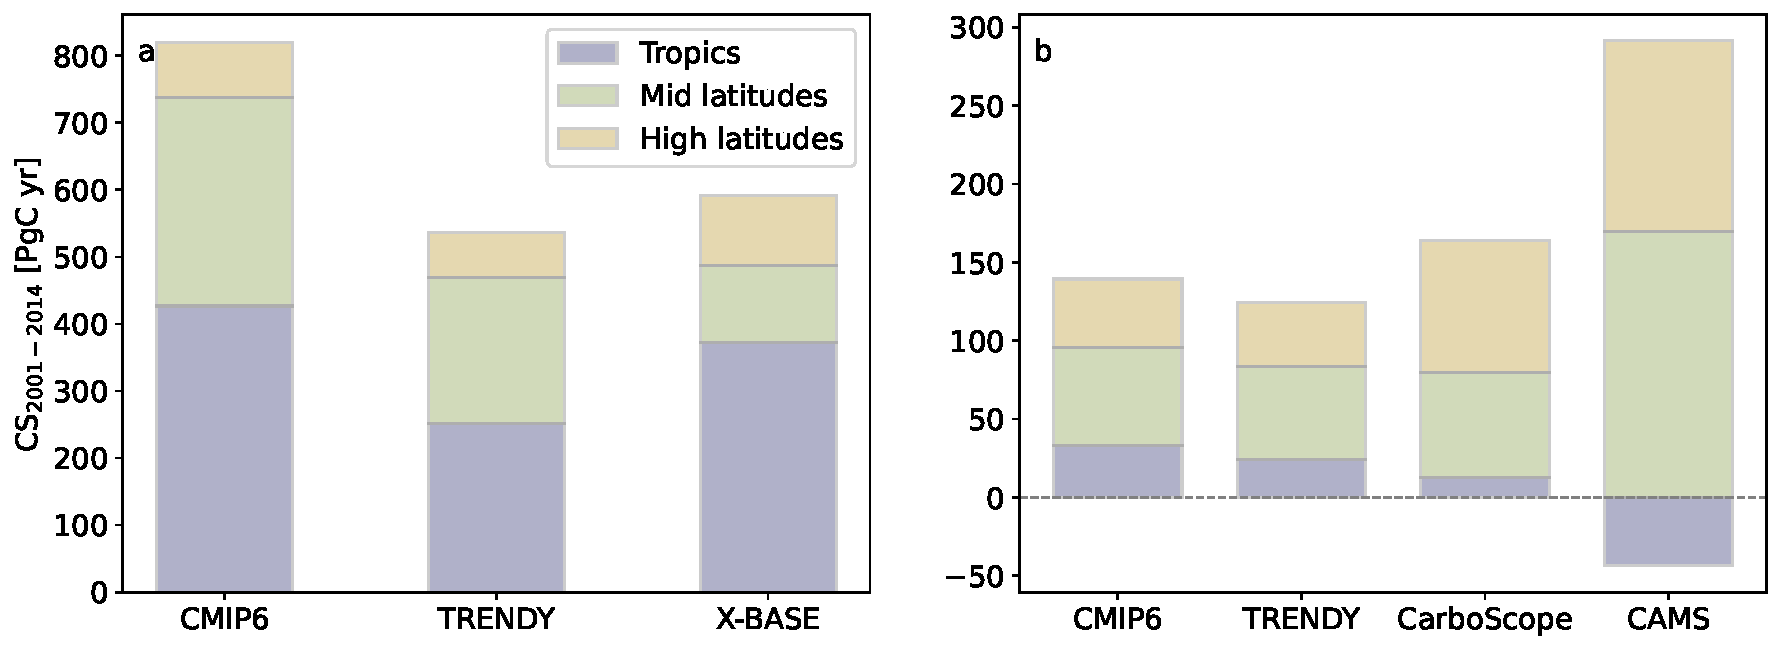
\includegraphics[width=1.0\linewidth]{Images/Comparison_NEPvsNBP_res.pdf}
    \caption{Carbon sequestration (CS) across different products (2001--2014) calculated using NEP or NEE (a) and NBP (b) and contributions of latitudinal zones (colors). The dotted lines in b indicate null values of CS. Negative (positive) values of CS indicate carbon debts (surpluses). CMIP6 and TRENDY CS values correspond to the weighted ensemble of their respective models. Note that the y-axis of a and b are on a different numerical range. To ensure a consistent comparison across all datasets, uncertainty envelopes are omitted. While the multi-model ensembles possess a raw internal spread, CarboScope, CAMS, and X-BASE provide deterministic values from which a statistical error cannot be derived.}
    \label{fig:all_products}
\end{figure}

When comparing all four products with NBP results (CMIP6, TRENDY, CarboScope, and CAMS) over their common period (2001-2014, Fig.~ \ref{fig:all_products}b), CAMS shows the largest CS deviations relative to the other datasets. The CarboScope and CAMS products suggest an overestimation of CS by CMIP6 and TRENDY ensembles in the tropics and underestimations in high latitudes. 
In tropical regions, the marked reduction from NEP-based to NBP-based CS during these 14 years is consistent across both model ensembles: CMIP6 drops from 427~PgC~yr (NEP) to 33~PgC~yr (NBP) (394~PgC~yr difference), while TRENDY decreases from 252~PgC~yr to 24~PgC~yr (228~PgC~yr difference; Table~S4). This difference far exceeds that observed in other latitudes, driving the pronounced global differences between CS based on NEP versus NBP. 

\section{Discussion}
\subsection{Trade-off between carbon assimilation and lagged respiratory responses}
Our approach to computing Carbon Sequestration (CS) as the double integral of carbon exchange between terrestrial ecosystems and the atmosphere enables the evaluation of long-term tradeoffs between carbon assimilation and lagged respiration responses. This approach implicitly incorporates the transit time of carbon through terrestrial ecosystems and quantifies the cumulative effects of the delayed release of carbon fluxes from ecosystems back to the atmosphere (see \ref{sec:appCS}). This is in contrast to simply analyzing changes in carbon stocks, which do not appropriately account for lagged respiration effects from previous carbon legacies (Fig.~S10). A recent study using a similar methodology has demonstrated its applicability for analyzing long-term carbon dynamics and how CS is connected to the transient climate response to cumulative emissions (TCRE) \citep{Matthews2023}. High Carbon Sequestration arises from either high assimilation rates, as in tropical latitudes, or slow respiration responses, characteristic of high latitudes (Figs.~S1 and S2). Here, we found that the assimilation effect dominates globally over the lagged respiration effect. Therefore, the tropics emerged in our analysis as the region with the greatest potential to simultaneously retain large amounts of carbon for longer periods, over decadal to centennial timescales, in the absence of disturbances (Figs.~\ref{fig:CS_NEP} and \ref{fig:CMIP6_TRENDY_NEP_time}). 

The monotonic increasing trend in NEP-based CS across X-BASE, CMIP6, and TRENDY models is mostly driven by larger GPP than respiration fluxes ($r_h+r_a$) in all regions over the simulation time-frames (Figs.~\ref{fig:CS_NEP}c, \ref{fig:CMIP6_TRENDY_NEP_time}a,c, S1 and S2). This pattern could represent an artifact of models or a real sustained carbon sink due to CO$_2$ and N fertilization, increased water use efficiency, or prolonged growing season \citep{Fernandez-Martinez2017,Fernandez-Martinez2019,OSullivan2019,Friedlingstein2023,Ruehr2023}. Regardless of the underlying driver, the key insight from our results is that as long as GPP increases monotonically, the lagged respiration response of the biosphere does not catch up. Consequently, substantial quantities of carbon are retained over time within terrestrial ecosystems, remaining out of the atmosphere. However, this sustained monotonic increase in NEP-based CS does not yet account for additional losses such as fires, land-use change, and other emissions included in NBP, which can completely change CS trajectories.


\subsection{Consequences of disturbances}
Factors beyond climate, such as deforestation and fires, significantly reduce CS values. While localized natural disturbances such as wildfires or storms inherently drive transient negative CS balances, a persistent, long-term carbon debt emerges primarily when anthropogenic activities artificially amplify these disturbance-driven carbon losses or prevent ecosystem recovery \citep{de-Miguel2025,Turetsky2015}. Long-term simulations from 1850 to 2014 by most CMIP6 and TRENDY models indicate cumulative carbon releases exceeding assimilation (Fig.~\ref{fig:CMIP6_TRENDY_NBP_time}), placing terrestrial ecosystems in net carbon debt relative to pre-industrial carbon stocks. These debts are not fully apparent when using data-driven products (Fig.~\ref{fig:CS_NBP}c,f). While these datasets implicitly reflect the present-day flux consequences of past legacy effects, their short temporal horizon prevent integrating the CS metric over the full historical trajectory required to fully capture older historical disturbances. 

Mid-latitude zones exhibit particularly large negative CS, leading to a substantial global carbon debt. This debt has grown since the beginning of the Industrial Revolution (Fig.~\ref{fig:CMIP6_TRENDY_NBP_time}), mostly driven by large release fluxes in tropical and mid-latitude regions (Fig.~S1 and S2). After the 1970s, CS shows signs of recovery as mid-latitude forest regrowth partially offsets the debt. 
Nevertheless, CMIP6 and TRENDY ensembles indicate that by 2014, the carbon debt remained substantial, particularly in regions such as Eastern North America, Central America, the Northern Andes, and Eastern South America (Fig.~S8 and S9).

Differences between NEP- and NBP-based CS highlight the critical role of disturbances on the biosphere's capacity to fix carbon out of the atmosphere and retain it for long periods (Fig.~\ref{fig:CS_NEP}c vs. Fig.~\ref{fig:CS_NBP}c,f and Fig.~\ref{fig:CMIP6_TRENDY_NEP_time} vs. Fig.~\ref{fig:CMIP6_TRENDY_NBP_time}). These differences are particularly pronounced in the tropics, where high carbon fixation amounts are counteracted by substantial release fluxes from deforestation and other disturbances, hindering the ability of these regions to retain carbon over decadal timescales. Empirical studies report that respired carbon in tropical forests has a mean age in the order of a few years up to two decades \citep{Sierra2021JE,Chanca2025}. This implies that lagged respiration effects in the tropics are intrinsically rapid and can be exacerbated by additional losses due to disturbances, which would drastically reduce transit times. Consequently, when evaluated using the CS metric, the carbon loss over time in tropical regions significantly exceeds that of other latitudinal zones. 

When analyzing the periods 2001--2019 (Fig.~\ref{fig:CS_NBP}c,f) and 2001--2014 (Fig.~\ref{fig:all_products}b), CS calculated with NBP shifts to positive values, albeit remaining substantially lower than CS-based NEP for the same periods (Fig.~\ref{fig:CS_NEP}c and \ref{fig:all_products}a). This shift in the trend of CS demonstrates how carbon flux balances can vary significantly depending on the chosen time horizon: over these 14 or 19 years, carbon inputs can offset recent losses. However, these short-term gains are insufficient to counteract the long-term accumulated historical carbon debts. This temporal sensitivity is further illustrated by the rolling-window CS calculations (Fig.~S13). For NEP-based metrics, the mean CS value increases consistently with wider integration windows. Conversely, for NBP-based metrics, the sign of CS switches depending on the window length. Over several decades, wider integration windows lead to deeper negative values in debt-prone regions, yet yield higher positive values in carbon-surplus areas. Notably, for both metrics, the spatial standard deviation decreases as the integration window expands.

\subsection{Discrepancies among products and models, and limitations of CS}
All products show similar trends during the overlapping period (Fig.~\ref{fig:all_products}), with tropical regions exhibiting the highest NEP-based CS and largest discrepancies for NBP-based CS.  It is well documented that models and data-driven products generally perform worse in the Global South, where observational constraints are sparse and ecosystems are highly heterogeneous \citep{Gier2024}. Nevertheless, the high spatial consistency across all datasets confirms a robust global pattern of carbon sequestration, even if their magnitudes remain uncertain.

Discrepancies in net magnitudes arise from their underlying methodologies, which contributes to the observed spread in NBP-based CS observation-driven inversions (CarboScope, CAMS) infer a net land flux that is consistent with atmospheric CO$_2$ measurements and a prescribed prior, whereas X-BASE upscales site-level NEE using machine learning trained on eddy-covariance data and remote-sensing predictors. In contrast, CMIP6 ESMs and TRENDY DGVMs explicitly simulate carbon fluxes using diverse mathematical formulations such as specific fire modules, wood harvest pools and land-cover conversion pathways. As a result, the disturbance fluxes included in CMIP6 and TRENDY vary widely among models. This heterogeneity makes it difficult to isolate which specific disturbance processes are responsible for the carbon debts identified in different regions.

Observation-based products are generally more reliable than process-based models (e.g., CMIP6, TRENDY) because atmospheric CO$_2$ observations directly constrain net fluxes, avoiding ecosystem process parameterization biases %, and match independent aircraft data well 
\citep{Gaubert2019,Woude2025}. However, their short temporal coverage fails to fully capture long-term carbon legacies resolved by process models.

Multi-model intercomparison initiatives like CMIP6 and TRENDY include numerous models, complicating the identification of the most reliable individual model. While previous studies show that simple multi-model averages often agree better with observations than single models, equal weighting proves inappropriate for climate science inference \citep{Hagedorn2005,Knutti2017}. This motivates our use of grid-cell-level weighted ensemble averaging, where weights represent the probability of each model being the best performer locally against observational benchmarks \citep{Sierra2025GDM}. These spatially variable weights reduce bias from outlier models and yield lower prediction uncertainty than arithmetic means. However, our ensemble approach may incur in several limitations. Model weights are static in time, estimated over the overlap period with observational products and held fixed thereafter; this assumes that relative performance during the calibration window is representative of other periods and precludes dynamic adjustment to changing climate, land use, or multi-decadal phases. Nevertheless, the traditional equal weight approach also assumes constant equal weights for the entire averaging period, so our assumption of constant weights is not worse than other model averaging approaches. 
Another potential limitation is that the weighting scheme treats models as independent, ignoring structural dependencies and shared biases arising from common parameterizations, forcing data, or model families, and it lacks an explicit penalty for model complexity as required in formal information-theoretic frameworks. In addition, a key underlying assumption of this approach is that data-driven products, such as X-BASE, accurately represent real-world benchmarks, though they carry structural uncertainties, including regional artifacts like artificially high NEE values in areas such as India. These local biases can misguide ensemble optimization by overweighting models that replicate spatial artifacts or penalizing those with stronger interannual climate sensitivity. Consequently, we recommend that future studies utilize updated and refined versions of X-BASE and other data products to recalculate and validate these weighted multi-model ensembles when they become available.

\subsection{Implications for climate-change mitigation policies}

The CS metric integrates both the amount of carbon and the time it is retained, offering a robust framework for improving and supporting carbon accounting protocols in nature-based mitigation programs, such as the Reducing Emissions from Deforestation and Forest Degradation in Developing Countries (REDD+) or other policies from the United Nations Framework Convention on Climate Change. CS increases as carbon is retained for longer times; therefore, it can be used to generate incentives for land management actions that promote the preservation of carbon storage over time. 

By incorporating the time component into the quantification of carbon sequestration, our analysis reveals the importance of explicitly defining temporal boundaries to assess the long-term carbon balance between the land and the atmosphere. Assessing Carbon Sequestration for recent and short integration times misses the importance of historical trends in carbon exchange. Human activity has disrupted the global carbon cycle mostly since the beginning of the Industrial Revolution, generating an important historical debt. Consequently, targets for global carbon-management policies must prioritize repaying this debt, as inaction will amplify its magnitude over time or allow only a very slow recovery, as seen during the last few decades.

The tradeoff between carbon assimilation and release over long timescales from multiple models and observation-based products suggests that tropical regions play a critical role in assimilating and retaining carbon over time, but this capacity has been disrupted drastically by historical changes in land use, particularly deforestation \citep{Li2022}. This capacity also hints at the significant potential for increasing the carbon retention time in tropical regions through reduced disturbance levels and large-scale restoration of deforested areas. Such measures could repay a substantial share of the considerable terrestrial biosphere's carbon debt relative to pre-industrial global carbon stocks.

Our analysis also suggests that terrestrial ecosystems can only act as significant and long-term (decades to centuries) sinks of anthropogenic carbon as long as assimilation increases monotonically over time, so lagged release effects do not have enough time to compensate for the increase in assimilation. However, this scenario seems unlikely for the future of the global carbon cycle, either because of a saturation effect of carbon assimilation resulting from multiple limitations \citep{Melnikova2021,Friedlingstein2023}, or because of an increase in the frequency and intensity of disturbances in terrestrial ecosystems \citep{Xu2021,Sitch2024}.

\section{Conclusions}\footnote{The contrast between NEP- vs NBP-based CS is missing from this final conclusion statement. The reviewer highlighted this as one of the main results, and I think it should be reflected somehow here in the conclusions. }

The CS metric offers a robust framework for policies that incentivize long-term land management to sustain carbon storage, as it integrates carbon amount and the time it is retained. Historical analyses reveal that tropical regions contribute the most to terrestrial carbon retention in the absence of disturbances; however, human activities have created substantial pre-industrial carbon debt, driven primarily by tropical deforestation. This underscores the need to address legacy imbalances when setting global climate targets. Consequently, tropical regions hold key potential for recovering the large global carbon debt accumulated since pre-industrial times. Incentives to recover this debt may be achieved by accounting for the time that carbon is preserved in natural ecosystems and remains out of the atmosphere, where it would contribute to radiative forcing. Furthermore, the choice of a specific time horizon fundamentally shapes our conclusions, underscoring the importance of accounting for carbon legacies. Overall, integrating time as a variable in carbon sequestration assessments can help us to effectively quantify tradeoffs between carbon assimilation and release, forecast timelines for historical carbon debt repayment under recovery scenarios, and better define policy instruments for climate change mitigation.

% evidence from multiple products considering the historical record of carbon exchange between the land and the atmosphere suggests that long-term global Carbon Sequestration is driven predominantly by the large assimilation fluxes in tropical regions, which dominate over their fast-release fluxes. However, the ability of the tropics to retain carbon over time has been disrupted dramatically since the beginning of the Industrial Revolution by land-use changes and fire regimes. At the same time, the tropics may be key to recovering the large global carbon debt accumulated since pre-industrial times. Incentives to recover this debt may be achieved by accounting for the time that carbon is preserved in natural ecosystems and remains out of the atmosphere, where it would contribute to radiative forcing. Overall, integrating time as a variable in carbon sequestration assessments can help us to effectively quantify tradeoffs between carbon assimilation and release, forecast timelines for historical carbon debt repayment under recovery scenarios, and better define policy instruments for climate change mitigation.


\begin{acknowledgements}[Acknowledgements]
We acknowledge the CMIP community for providing the climate model data, stored and globally distributed in the framework of the ESGF. The CMIP data used in this study were replicated and made available by the Deutsches Klimarechenzentrum (DKRZ). Also, we thank the developers of the CAMS, X-BASE, and the Jena CarboScope (C. Rödenbeck) products for publishing their results in an open platform.

\end{acknowledgements}

\appendix
% \renewcommand{\thesection}{A\arabic{section}}
\section{Carbon Sequestration CS and transit times} 
\label{sec:appCS}
The concept of carbon sequestration in ecosystems is closely linked to the concept of the transit time of carbon. In terrestrial ecosystems, we define the transit time of carbon as the amount of time that it takes for carbon atoms to pass through an entire ecosystem, from photosynthesis until respiration by autotrophs and heterotrophs. 
%At a particular time $t$, the time a certain amount of carbon has remained in the system since its arrival at time $t'$ is its age $a=t-t'$.
Because carbon sequestration is not only about the amount of carbon that enters an ecosystem but also about how long it remains stored there, we need an approach that quantifies and combines transit times with the amount of carbon entering ecosystems. Previous works by \citet{Sierra2021} and \citet{Metzler2024} introduced a set of definitions integrating transit times with carbon mass. 
Here, we present the connections between transit time and carbon mass, $\CS$ as used here, and their underlying theory in carbon transit times.


\subsection{The terrestrial biosphere as a non-autonomous compartmental system}
We can model the carbon stocks and fluxes within, into, and from the terrestrial biosphere as a $d$-dimensional non-autonomous compartmental system that can be described by the vector-valued ordinary differential equation (ODE) 
\begin{equation}
    \label{eqn:comp_sys}
    \begin{aligned}
        \frac{\mathrm{d}}{\dd{t}}\,\vec{C}(t) &= \tens{B}(t)\,\vec{C}(t) + \vec{s}(t),\quad t>t_0,\\
        \vec{C}(t_0) &= \vec{C}_0,
    \end{aligned}
\end{equation}
where $\vec{C}(t)$ is the vector of carbon stocks at time $t$ in $\PgC$ with initial value $\vec{C}_0$ at initial time $t_0$, and $\vec{s}(t)$ is the vector of carbon input fluxes to the terrestrial biosphere coming from the atmosphere at time $t$ in $\PgCperyr$.
The compartmental-matrix-valued function $\tens{B}$ governs the carbon dynamics among the different compartments and carbon leaving the system.
Writing $\vec{1}^{\top}$ for the row vector comprising only ones,
\begin{equation}
    \vec{r}(t) = -\vec{1}^{\top}\,\tens{B}(t)\,\vec{C}(t)
\end{equation}
is the vector of carbon output fluxes from the terrestrial biosphere to the atmosphere at time $t$ in $\PgCperyr$.
The solution to \eqref{eqn:comp_sys} is given by
\begin{equation}
    \vec{C}(t) = \tens{\Phi}(t,t_0)\,\vec{C}_0 + \intl_{t_0}^t \tens{\Phi}(t,t')\,\vec{s}(t')\dd{t'},\quad t\geq t_0,
\end{equation}
with $\tens{\Phi}$ being the state transition operator of the compartmental system.
It is given as the solution to the matrix-valued ODE
\begin{equation}
    \begin{aligned}
        \frac{\mathrm{d}}{\dd{t}}\,\tens{\Phi}(t, t') &= \tens{B}(t)\,\tens{\Phi}(t, t'),\quad t>t',\\
        \tens{\Phi}(t',t') &= \tens{I}_d,
    \end{aligned}
\end{equation}
where $\tens{I}_d$ is the $d$-dimensional identity matrix.
The vector $\tens{\Phi}(t,t')\,\vec{s}(t')$ is the carbon vector of the system input $\vec{s}(t')$ at time $t'$ that is still in the system at time $t$.
Using the $l_1$-norm $\vnorm{\vec{v}} = \sum_{i=1}^d |v_i|$, the scalar functions $C(t):=\vnorm{\vec{C}(t)}$, $s(t):=\vnorm{\vec{s}(t)}$, $r(t):=\vnorm{\vec{r}(t)}$, and the nonnegative value $C_0=\vnorm{\vec{C}_0 }$ describe the total amounts of carbon stocks in the system at time $t$, the total carbon influx to the system, the total carbon outflux from the system, and the total initial carbon stock, respectively.

\subsection{System sojourn time}
If we define
\begin{equation}
    \itPhi(t,t', \vec{s}) := \tens{\Phi}(t, t')\,\vec{s}
\end{equation}
with $\tens{\Phi}$ being the state transition operator of system in Eq.~\noEqref{eqn:comp_sys}, then $\itPhi(t, t', \vec{s})$ is the amount of the system input $s:=s(t')=\vnorm{\vec{s}(t')}$ at time $t'\leq t$ that is still in the system at time $t$.
Note that $\itPhi$ is linear in $\vec{s}$ such that
\begin{equation}
    \itPhi(t,t',\vec{s_1}+\vec{s_2}) = \itPhi(t,t',\vec{s_1}) + \itPhi(t,t',\vec{s_2}).
\end{equation}
Now, divide $\vec{s}$ into $N$ equally small packages $\vec{s}_i=\vec{s}/N$ such that $\vec{s}=\sum_{i=1}^N \vec{s}_i$.
We make the packages $\vec{s}_i$ so small by choosing $N$ so large such that, for all $i\leq N$ and all $t\geq t'$, we have
\begin{equation}
    \itPhi(t, t', \vec{s}_i) = \mathit{\Psi}_i(t, t') \, s_i
\end{equation}
with $s_i=\vnorm{\vec{s}_i}$ and $\mathit{\Psi}_i(t, t') \in \{0, 1\}$.
This means that all particles of $s_i$ show the same future behavior after $t'$ in the sense that
\begin{equation}
    \mathit{\Psi}_i(t, t') = 
    \begin{cases}
        0, & \text{all particles of $s_i$ have left the system before time }t,\\
        1, & \text{all particles of $s_i$ are still in the system at time }t.
    \end{cases}
\end{equation}
By construction,
\begin{equation}
    \intl_{t'}^{t_0+T} \mathit{\Psi}_i(t, t')\dd{t}
\end{equation}
is the time that a single particle of $s_i$ spends in the system during the interval $[t',t_0+T]$ and
\begin{equation}
    s_i\intl_{t'}^{t_0+T} \mathit{\Psi}_i(t, t')\dd{t}
\end{equation}
is the mass-time ($\PgCyr$) that $s_i$ spends in the system.
Consequently,
\begin{equation}
    \begin{aligned}
        \intl_{t'}^{t_0+T} \itPhi(t',t,\vec{s}(t'))\dd{t} \\
        &= \intl_{t'}^{t_0+T} \itPhi\left(t,t',\sum_{i=1}^N \vec{s}_i\right)\dd{t} \\
        &= \intl_{t'}^{t_0+T} \sum_{i=1}^N \itPhi(t,t',\vec{s}_i)\dd{t} \\
        &= \intl_{t'}^{t_0+T} \sum_{i=1}^N \mathit{\Psi}_i(t,t')\,s_i\dd{t}\\
        &= \sum_{i=1}^N s_i\intl_{t'}^{t_0+T}\mathit{\Psi}_i(t,t')\dd{t}
    \end{aligned}
\end{equation}
describes the mass-time ($\PgCyr$) that all particles of the input $\vec{s}(t')$ spend in the system during the interval $[t',t_0+T]$.
We call this mass-time $\itPhi(t,t',\vec{s}(t'))$ the {\it system sojourn time} of $s(t')$.

\subsection{Carbon sequestration, system sojourn times, and transit times of compartmental systems}
In this section, we show how our definition of $\CS$ is related to the concepts 
{\it Integrated Net Carbon Balance} ($\INCB$), {\it Integrated Inputs Transit Time} ($\IITT$), and {\it Integrated Carbon Stocks} ($\ICS$) introduced in \citet{Metzler2024} and of which $\IITT$ is equivalent to {\it Carbon Sequestration} ($\CS$) as defined (differently from here) in \citet{Sierra2021}.
Except for $\INCB$, all of these concepts are connected to each other through the underlying concepts of system sojourn times or transit times.
Unfortunately, despite its lack of support by transit times, $\INCB$ is very often used as a metric for carbon sequestration.

More generally, we want to demonstrate that a family of metrics can effectively integrate the concepts of carbon inputs and transit times, allowing us to quantify the concept of carbon sequestration (\ref{tab:family_of_measures}).
The aspects of the general theory of forward transit times of non-autonomous compartmental systems that we present here originate from \citet{Metzler2018PNAS}.

The forward transit time $\tau(t')$ of a non-autonomous compartmental system is the time span that input entering the system at time $t'$ will spend in it before exiting.
The exit of a particle occurs at time $t$, with the particle's age at exit given by $a=t-t'$, where age measures the time since the particle's entry into the system.
This forward transit time has a density function $p_\tau(\cdot,t')$ such that $p_\tau(t-t',t')$ is the mass that enters the system at time $t'$ and leaves the system at time $t$, having spent the period $a=t-t'$ in the system.

For the compartmental system in Eq.~\noEqref{eqn:comp_sys}, this density is given by
\begin{equation}
    p_\tau(t-t', t') = -\vec{1}^{\top}\,\tens{B}(t)\,\tens{\Phi}(t, t')\,\vec{s}(t')
\end{equation}
and its cumulative distribution by
\begin{equation}
    \begin{aligned}
        P_\tau(t-t',t') &= \intl_0^{t-t'} p_\tau(a, t')\dd{a} = \vnorm{\vec{s}(t')} - \vnorm{\tens{\Phi}(t,t')\,\vec{s}(t')} \\
        &= s(t') - \itPhi(t,t',\vec{s}(t')).
    \end{aligned}
\end{equation}
The cumulative distribution $P_\tau(t-t',t')$ describes the mass that enters the system at time $t'$ and leaves the system younger than $t-t'$, hence before $t'$.
The survival function
\begin{equation}
    S_\tau(t-t',t'):=\vnorm{\vec{s}(\tau)} - P_\tau(t-t',t') = \vnorm{\tens{\Phi}(t,t')\,\vec{s}(t')} = \itPhi(t,t',\vec{s}(t'))
\end{equation}
describes the remaining amount at time $t$ from the input at time $t'$.
To make $p_\tau(\cdot,t')$, $P_\tau(\cdot,t')$, and $S_\tau(\cdot,t')$ probability density functions, cumulative distribution functions, and probabilistic survival functions, we need to normalize them by the total input amount $s(t')$ at time $t'$.
Defining $\vec{\beta}(t'):=\vec{s}(t')/s(t')$ to be the unit vector (in $l_1$-norm) that distributes the incoming carbon $s(t')$ at time $t$ to the different compartments, we obtain the normalized cumulative distribution function of $\tau(t')$ as
\begin{equation}
    F_\tau(t-t',t') = 1 - \vnorm{\tens{\Phi}(t,t')\,\vec{\beta}(t')}
\end{equation}
and its mean or expected value as
\begin{equation}
    \mathbb{E}\left[\tau(t')\right] = \intl_{t'}^\infty \left[1-F_\tau(t-t',t')\right]\dd{t} = \intl_{t'}^\infty \vnorm{\tens{\Phi}(t,t')\,\vec{\beta}(t')}\dd{t},
\end{equation}
and hence
\begin{equation}
    \intl_{t'}^\infty \vnorm{\tens{\Phi}(t,t')\,\vec{s}(t')}\dd{t} = s(t')\,\mathbb{E}\left[\tau(t')\right]
\end{equation}
as a weighted mean transit time.
Recalling $\itPhi(t,t',\vec{s}(t'))=\vnorm{\tens{\Phi}(t,t')\,\vec{s}(t')}$, we can interpret the system sojourn time of
$s(t')$, given by
\begin{equation}
    \intl_{t'}^{t_0+T} \itPhi(t,t',\vec{s}(t'))\dd{t} = \int_{t'}^{t_0+T} \vnorm{\tens{\Phi}(t,t')\,\vec{s}(t')}\dd{t},
\end{equation}
as a weighted {\it truncated mean forward transit time}.

Consequently, the {\it Integrated Inputs Transit Time} on the interval $[t_0, t_0+T]$, defined as
\begin{equation}
    \label{eqn:IITT}
    \begin{aligned}
        \IITT(t_0, T) &:= \intl_{t_0}^{t_0+T} \intl_{t'}^{t_0+T} \vnorm{\tens{\Phi}(t,t')\,\vec{s}(t')}\dd{t}\dd{t'} \\
        & = \intl_{t_0}^{t_0+T} \intl_{t'}^{t_0+T} \itPhi(t,t',\vec{s}(t'))\dd{t}\dd{t'},
    \end{aligned}
\end{equation}
represents the integrated weighted truncated mean forward transit times or the integrated system sojourn times of inputs to the system on the interval $[t_0, t_0+T]$.

$\IITT$ considers only the fate of carbon input to the system during the interval $[t_0,t_0+T]$ and ignores the fate of the initial carbon vector $\vec{C}_0$.
If we interpret $\vec{C}_0$ as a pulse input $\delta(t'-t_0)\,\vec{C}_0$ at time $t_0$, then we can extend $\IITT$ to
\begin{equation}
    \label{eqn:ICS}
    \begin{aligned}
        \intl_{t_0}^{t_0+T} \intl_{t'}^{t_0+T} &\vnorm{\tens{\Phi}(t,t')\,\left[s(t')+ \delta(t'-t_0)\,\vec{C}_0\right]}\dd{t}\dd{t'} \\
        &=\intl_{t_0}^{t_0+T} \delta(t'-t_0) \intl_{t'}^{t_0+T}\vnorm{\tens{\Phi}(t,t')\,\vec{C}_0}\dd{t}\dd{t'} \\
        &+ \intl_{t_0}^{t_0+T}\intl_{t'}^{t_0+T}\vnorm{\tens{\Phi}(t,t')\,\vec{s}(t')}\dd{t}\dd{t'}\\
        &= \intl_{t_0}^{t_0+T}\vnorm{\tens{\Phi}(t,t_0)\,\vec{C}_0}\dd{t} +\intl_{t_0}^{t_0+T}\intl_{t'}^{t_0+T}\vnorm{\tens{\Phi}(t,t')\,\vec{s}(t')}\dd{t}\dd{t'}\\
        & = \intl_{t_0}^{t_0+T}\vnorm{\tens{\Phi}(t,t_0)\,\vec{C}_0}\dd{t} + \intl_{t_0}^{t_0+T} \intl_{t_0}^t \vnorm{\tens{\Phi}(t,t')\,\vec{s}(t')}\dd{t'}\dd{t}\\
        &= \int_{t_0}^{t_0+T} \vnorm{\vec{C}(t)}\dd{t},
    \end{aligned}
\end{equation}
which equals the {\it Integrated Carbon Stocks} $\ICS(t_0,T)$, meaning, we can interpret $\ICS(t_0, T)$ as a weighted system sojourn time of all particles that at some time belong to the system during the interval $[t_0,t_0+T]$ or as weighted truncated mean forward transit time of all particles entering the system with the initial carbon stocks interpreted as a pulse input.

Considering the {\it Integrated Net Carbon Balance}
\begin{equation}
    \begin{aligned}
        \INCB(t_0,t) &= \intl_{t_0}^{t}\left[\vnorm{\vec{s}(t')}-\vnorm{\vec{r}(t')}\right]\dd{t'} \\
        &= \intl_{t_0}^t \left[s(t')-r(t')\right]\dd{t'} = C(t)-C_0,
    \end{aligned}
\end{equation}
we notice that the {\it Carbon Sequestration}
\begin{equation}
    \CS(t_0,T) = \intl_{t_0}^{t_0+T} \intl_{t_0}^t \left[s(t')-r(t')\right]\dd{t'}\dd{t}
\end{equation}
can be written as
\begin{equation}
    \begin{aligned}
        \CS(t_0,T)& = \intl_{t_0}^{t_0+T} \INCB(t_0,t)\dd{t}\\ 
        &= \intl_{t_0}^{t_0+T} \left[C(t) - C_0\right]\dd{t} = \ICS(t_0,T) - T\,C_0.
     \end{aligned}
\end{equation}
Notice that if we start with an empty system, i.e. $\vec{C}(t_0) = \vec{0}$, all metrics coincide, i.e.,  $\CS = \ICS = \IITT$. 
Similarly, if we compare $\CS$ for two different scenarios $A$ and $B$, both with the same initial carbon stock vector $\vec{C}(t_0)=\vec{C}_0$, then
\begin{equation}
    \label{eqn:Delta_CS}
    \begin{aligned}
        \Delta\CS(A,B)& := \CS_A(t_0,T) - \CS_B(t_0,T)\\ 
        &= \ICS_A(t_0,T) - \ICS_B(t_0,T)
    \end{aligned}
\end{equation}
and hence $\Delta\CS(A,B)$ is a comparison measure of two scenarios $A$ and $B$ based on weighted system sojourn times or weighted truncated mean forward transit times.

In summary, the family of metrics IITT, ICS, and CS are different forms of mean forward transit times integrated over time and truncated until the time of observation. Their main difference is the way they treat the legacy carbon from the initial conditions. One of the main advantages of using these metrics is that they combine both the amount of carbon and the time it remains stored in a compartmental system without the need to explicitly calculate transit times. We believe these metrics are essential to quantify the more general concept of carbon sequestration because they account for how much of the total carbon that enters a system will be retained for a period of time, potentially including legacy effects from previously stored carbon. 

% \begin{table*}[t]
% \caption{A family of carbon sequestration metrics. $\IITT$ is constructed... (first part of caption)}
% \begin{center}
% \begin{tabular}{m{3cm} m{4cm} m{4cm} m{4cm}}
% \toprule
% \multicolumn{1}{c}{} & 
% \multicolumn{1}{c}{\textbf{Integrated Inputs Transit Time}} & 
% \multicolumn{1}{c}{\textbf{Integrated Carbon Stocks}} & 
% \multicolumn{1}{c}{\textbf{Carbon Sequestration}} \\
% \midrule
% \textbf{Computation} &
%     $\begin{array}{c} \displaystyle \IITT(t_0,T) = \intl_{t_0}^{t_0+T} \intl_{t'}^{t_0+T} \vnorm{\tens{\Phi}(t,t')\,\vec{s}(t')}\dd{t}\dd{t'} \\ \displaystyle = \intl_{t_0}^{t_0+T} \intl_{t'}^{t_0+T} \itPhi(t,t',\vec{s}(t'))\dd{t}\dd{t'} \end{array}$ &
%     $\begin{array}{c} \displaystyle \ICS(t_0,T) = \intl_{t_0}^{t_0+T} \vnorm{\vec{C}(t)}\dd{t} \\ \displaystyle = \intl_{t_0}^{t_0+T} C(t)\dd{t} \end{array}$ &
%     $\begin{array}{c} \displaystyle \CS(t_0,T) = \intl_{t_0}^{t_0+T} \intl_{t_0}^t \left[s(t')-r(t')\right]\dd{t'} \dd{t} \\ \displaystyle = \intl_{t_0}^{t_0+T} \left[C(t) - C_0\right]\dd{t} \end{array}$ \\
% \bottomrule
% \end{tabular}
% \end{center}
% \label{Table:family_of_measures_part1}
% \end{table*}

% RIGHT BEFORE your table in annex
\setcounter{table}{0}
\renewcommand{\thetable}{Table A\arabic{table}}

\begin{table*}[t]
    \caption{A family of carbon sequestration metrics. $\IITT$ is constructed directly on transit times, $\ICS$ extends $\IITT$ by interpreting the initial stocks as a pulse input, and $\CS$ allows comparison of different scenarios with equal initial total carbon stocks by having only fluxes available. In the case of an empty initial system, $C_0=0$, the three metrics coincide.}
    \centering
    \begin{tabular}{p{2cm} p{4cm} p{4cm} p{4cm}}
        \toprule
        & \textbf{Integrated Inputs Transit Time} & \textbf{Integrated Carbon Stocks} & \textbf{Carbon Sequestration} \\
        \midrule
        \textbf{Computation} &
        {\small
        \begin{minipage}{4cm}\centering
        $\IITT(t_0,T) = \intl_{t_0}^{t_0+T} \intl_{t'}^{t_0+T} \vnorm{\tens{\Phi}(t,t')\,\vec{s}(t')} \dd{t} \dd{t'}$ \\[2pt]
        $= \intl_{t_0}^{t_0+T} \intl_{t'}^{t_0+T} \itPhi(t,t',\vec{s}(t')) \dd{t} \dd{t'}$ \\[2pt]
        $= \ICS - \intl_{t_0}^{t_0+T} \vnorm{\tens{\Phi}(t,t_0)\,\vec{C}_0} \dd{t}$
        \end{minipage}
        } &
        {\small
        \begin{minipage}{4cm}\centering
        $\ICS(t_0,T) = \intl_{t_0}^{t_0+T} \vnorm{\vec{C}(t)} \dd{t}$ \\[2pt]
        $= \intl_{t_0}^{t_0+T} C(t) \dd{t}$ \\[2pt]
        $= \IITT + \intl_{t_0}^{t_0+T} \vnorm{\tens{\Phi}(t,t_0)\,\vec{C}_0} \dd{t}$
        \end{minipage}
        } &
        {\small
        \begin{minipage}{4cm}\centering
        $\CS(t_0,T) = \intl_{t_0}^{t_0+T} \intl_{t_0}^t [s(t')-r(t')] \dd{t'} \dd{t}$ \\[2pt]
        $= \intl_{t_0}^{t_0+T} [C(t) - C_0] \dd{t}$ \\[2pt]
        $= \ICS - T\,C_0$
        \end{minipage}
        } \\
        \midrule
     \textbf{\shortstack{Computational\\requirements}} & 
        {\small
        \begin{minipage}{4cm}\raggedright
             $\bullet$ State transition operator $\tens{\Phi}$ and influx vector $\vec{s}(t)$ through time; \\[1pt]
            $\bullet$ or $\ICS$ requirements and state transition operator $\tens{\Phi}$ through time.
        \end{minipage}
        } &
        {\small
        \begin{minipage}{4cm}\raggedright
            $\bullet$ Total carbon stocks $C(t)$ through time; \\[1pt]
            $\bullet$ or $\IITT$ requirements and initial carbon stock vector $\vec{C}(t_0)$.
        \end{minipage}
        } &
        {\small
        \begin{minipage}{4cm}\raggedright
            $\bullet$ Total influx $s(t)$ and outflux $r(t)$ through time; \\[1pt]
            $\bullet$ or total net influx through time; \\[1pt]
            $\bullet$ or total carbon stocks $C(t)$ through time.
        \end{minipage}
        } \\
        \midrule 
        \textbf{\shortstack{Connection to\\transit times} } & 
        Directly by construction as shown in~\eqref{eqn:IITT}. & 
        By interpretation as $\IITT$ extended to the initial stock vector $\vec{C_0}$ as a pulse input. & 
        By relative comparison in a scenario setup as shown in~\eqref{eqn:Delta_CS}. \\
        %\bottomrule
        \midrule 
    \end{tabular}
    \label{tab:family_of_measures}
\end{table*}







\begin{fundinginfo}[Funding information]
%This project has received funding from the European Union’s Horizon 2020 research and innovation programme under the Marie SkłodowskaCurie grant agreement No 101110350 (DISEQ - The Drought Impact on the Climate Benefit of Carbon Sequestration). The Max Planck Society has provided additional funding. M.F-M was supported by the European Research Council project ERC-StG-2022-101076740-STOIKOS and the Ramón y Cajal fellowship (RYC2021-031511-I) funded by the MICIU/AEI /10.13039/501100011033 and by FSE+. EK was supported by the ERTDF (JPMEERF24S12206) of the ERCA by MOE Japan. TN was supported by the German Federal Ministry of Education and Research (BMBF), project STEPSEC (Grant No. 01LS2102A). GH and LM were supported by NASA-CMS grants 80NSSC21K1059 and 80NSSC25K7221.
\end{fundinginfo}

\eject
\begin{authoraff}[AUTHOR AFFILIATIONS]


\end{authoraff}

\bibliographystyle{apa}
\bibliography{biblio}


\label{endPage_Label}
%\clearpage
\end{document} 